% !TEX program = xelatex
% 编译：在本目录执行 bash build.sh；成品输出到 ../report.pdf。
\documentclass{article}
\usepackage[
  paperwidth=595.3bp,
  paperheight=841.9bp,
  margin=0bp
]{geometry}
\usepackage{fontspec}
\usepackage{xeCJK}
\usepackage{pdfpages}
\usepackage{tikz}
\pagestyle{empty}
\setlength{\parindent}{0pt}

% 正文按原模板使用仿宋，页眉使用宋体。
% 本机优先使用 WPS 字体；其他系统可使用 TeX Live 自带的 Fandol。
\IfFileExists{/Applications/wpsoffice.app/Contents/Resources/office6/fonts/FangS-SC.ttf}{
  \setCJKmainfont{FangS-SC.ttf}[
    Path=/Applications/wpsoffice.app/Contents/Resources/office6/fonts/]
}{
  \setCJKmainfont{FandolFang-Regular.otf}
}
\IfFileExists{/Applications/wpsoffice.app/Contents/Resources/office6/fonts/ShuS-SC.ttf}{
  \newCJKfontfamily\headerfont{ShuS-SC.ttf}[
    Path=/Applications/wpsoffice.app/Contents/Resources/office6/fonts/]
}{
  \newCJKfontfamily\headerfont{FandolSong-Regular.otf}
}
\IfFontExistsTF{Times New Roman}{
  \setmainfont{Times New Roman}
}{
  \setmainfont{texgyretermes-regular.otf}
}
\xeCJKsetup{PunctStyle=plain, CJKglue=\hskip 0pt, CJKecglue=\hskip 0pt}

% 所有坐标单位为 PDF 的 bp，原点是页面左上角。
% 固定坐标保留原模板的边框、分页和留白；删字后不压缩表格。
\newcommand{\TemplateText}[4]{%
  \node[anchor=base west, inner sep=0pt, outer sep=0pt]
    at (#1,#2) {\fontsize{#3bp}{#3bp}\selectfont #4};%
}
\newcommand{\TemplateHeading}[3]{%
  \TemplateText{#1}{#2}{14.05}{#3}%
}
\newcommand{\TemplateRule}[1]{%
  \draw[line width=0.48bp] (84.91,#1) -- (510.39,#1);%
}
\newcommand{\TemplateSides}[1]{%
  \draw[line width=0.48bp] (85.15,72.0) -- (85.15,#1);
  \draw[line width=0.48bp] (510.15,72.0) -- (510.15,#1);%
}
\newenvironment{templatepage}{%
  \clearpage
  \null
  \begin{tikzpicture}[
    remember picture, overlay,
    shift={(current page.north west)},
    x=1bp, y=-1bp
  ]
    \TemplateText{397.44}{51.29}{9}{\headerfont《数字逻辑设计》实验报告}
    \fill (89.85,55.25) rectangle (505.45,55.97);
}{%
  \end{tikzpicture}
  \par
}

% 填写正文时可用此命令，在指定区域放入自动换行的文字。
% 参数依次为：左边距、顶部坐标、宽度、内容。单位均为 bp。
% 示例：\ReportContent{90.6}{123}{414}{这里填写功能描述。}
% 该命令不会自动扩展表格；长报告可自行调整边框坐标或新增页。
\newcommand{\ReportContent}[4]{%
  \node[
    anchor=north west, inner sep=0pt, outer sep=0pt,
    text width=#3bp, align=justify
  ] at (#1,#2) {\fontsize{12bp}{18bp}\selectfont #4};%
}

\begin{document}

% 封面是原 PDF 第 1 页的矢量副本，不重排、不截图、不改写。
% 原 PDF 第 2 页不纳入报告。
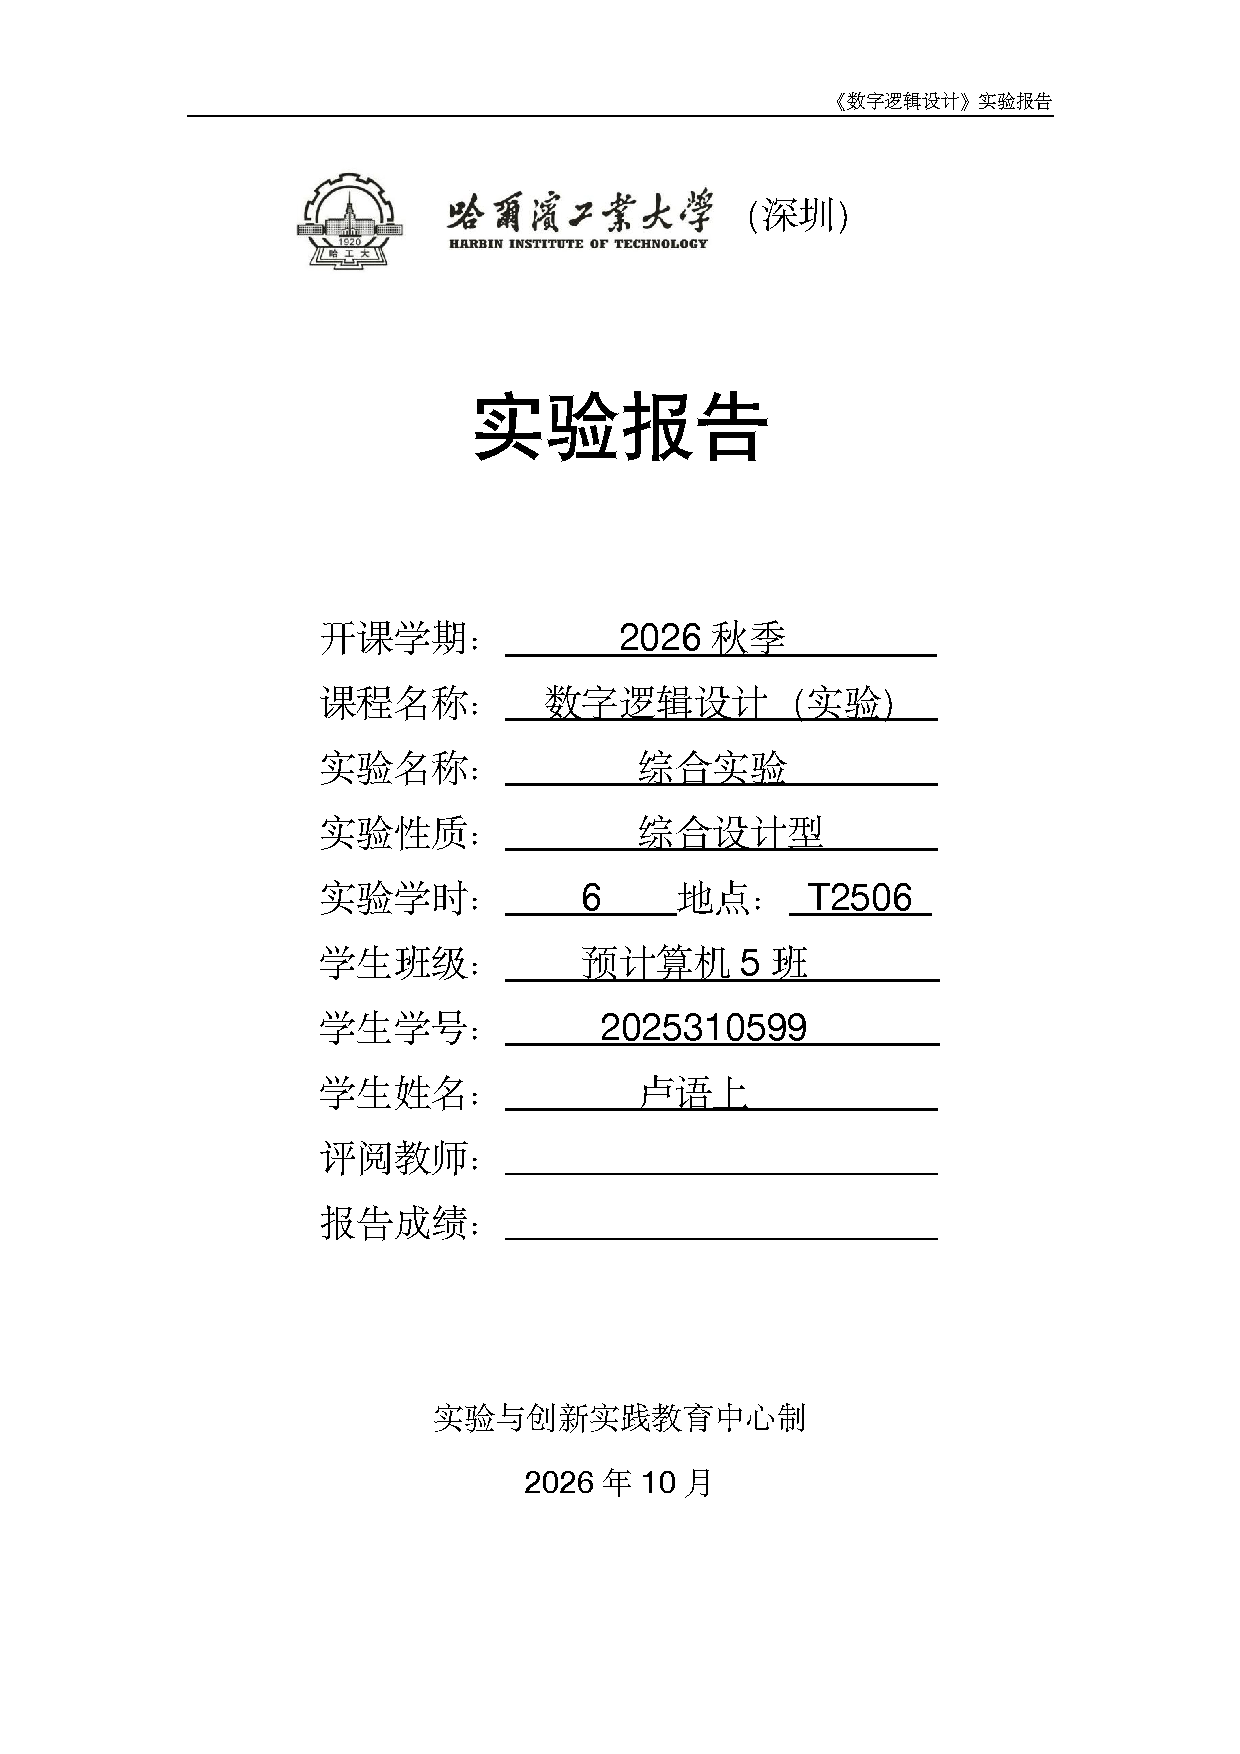
\includepdf[pages=1, fitpaper=true, noautoscale=true, pagecommand={}]{assets/cover.pdf}

% 原模板第 3 页：只保留黑色标题、黑色说明和表格线。
\begin{templatepage}
  \TemplateRule{72.24}
  \TemplateRule{103.94}
  \TemplateRule{217.24}
  \TemplateRule{248.94}
  \TemplateRule{577.04}
  \TemplateRule{608.74}
  \TemplateRule{765.14}
  \TemplateSides{764.90}

  \TemplateHeading{248.64}{93.17}{设计的功能描述}
  \TemplateText{90.60}{116.33}{12}{概述基本功能}
  % 在此填写功能描述。

  \TemplateHeading{269.64}{238.13}{系统设计}
  \TemplateText{90.60}{261.29}{12}{用硬件框图描述系统主要功能及各模块之间的相互关系}
  % 在此放置自己的系统框图与说明。

  \TemplateHeading{248.64}{597.89}{模块设计与实现}
  \TemplateText{90.60}{621.169}{12}{各子模块设计思路及实现}
  % 在此填写模块设计，下一页顶部保留原模板的续写区域。
\end{templatepage}

% 原模板第 4 页。
\begin{templatepage}
  \TemplateRule{72.24}
  \TemplateRule{244.34}
  \TemplateRule{279.64}
  \TemplateRule{420.54}
  \TemplateRule{455.84}
  \TemplateRule{737.04}
  \TemplateSides{736.80}

  % 顶部空白区域延续上一页的“模块设计与实现”。

  \TemplateHeading{269.64}{265.25}{仿真调试}
  \TemplateText{90.60}{292.009}{12}{仿真波形截图及仿真分析}
  % 在此填写仿真调试内容。

  \TemplateHeading{158.159}{441.409}{设计过程中遇到的问题及解决方法、Lint 分析}
  % 在此填写问题、解决方法和 Lint 分析。
\end{templatepage}

% 原模板第 5 页。
\begin{templatepage}
  \TemplateRule{72.24}
  \TemplateRule{107.54}
  \TemplateRule{295.24}
  \TemplateRule{330.54}
  \TemplateRule{449.14}
  \TemplateSides{448.90}

  \TemplateHeading{246.48}{93.05}{AI 工具使用总结}
  % 在此填写 AI 工具使用总结。

  \TemplateHeading{255.60}{316.13}{课程设计总结}
  % 在此填写课程设计总结。
\end{templatepage}

\end{document}
